%\ihead{\headmark}
\chapter{Deep Learning}

Deep learning is a subfield of machine learning which is a subfield of artificial intelligence (AI). Deep learning has emerged as one of the most exciting fields in computer science, and it keeps expanding its scope to some other domains as well. It can be used in many applications, such as medicine for identifying diseases, automatic game playing, self-driving cars, image recognition, and natural language processing. Deep learning is successful in many different domains because of its ability to understand multiple levels of representation of data. Its mean that it has not only the ability to classify and predict, but also the ability to learn a different level of complexity. Before directly jumping into deep learning, it is necessary to provide the concept of ``machine learning''.

\section{Machine Learning}

Machine learning is a data analysis method \cite{bishop2006pattern}. It gives the computer the ability to learn from data without being explicitly instructed. By using different machine learning algorithms, it helps to find hidden insights of data and allows us to build models for predictions. It can be classified into 2 categories \cite{machinelearningmastery}: supervised learning, and unsupervised learning.


\subsection{Supervised Learning}

In supervised learning, the labeled data is used to train the models. The labeled data represents the well known input and output variables. Thus, a supervised machine learning algorithm is used to as a function to map the input variables to output variables. Learning is supposed to be stopped when the level of performance reaches the desired result. Supervised learning is generally divided into regression and classification.
\begin{itemize}
	\item \textbf{Regression}: A problem in which the output variable is a category.
	\item \textbf{Classification}: A problem in which the output variable is the real value.
\end{itemize}

In supervised learning, the basic workflow is to build a model, evaluate or tune a model and then deploy it in the production environment, where it will make the predictions. The workflow can be seen in Figure \ref{fig:basic-ml-model}.


\begin{figure}[htpb]
	\centering
	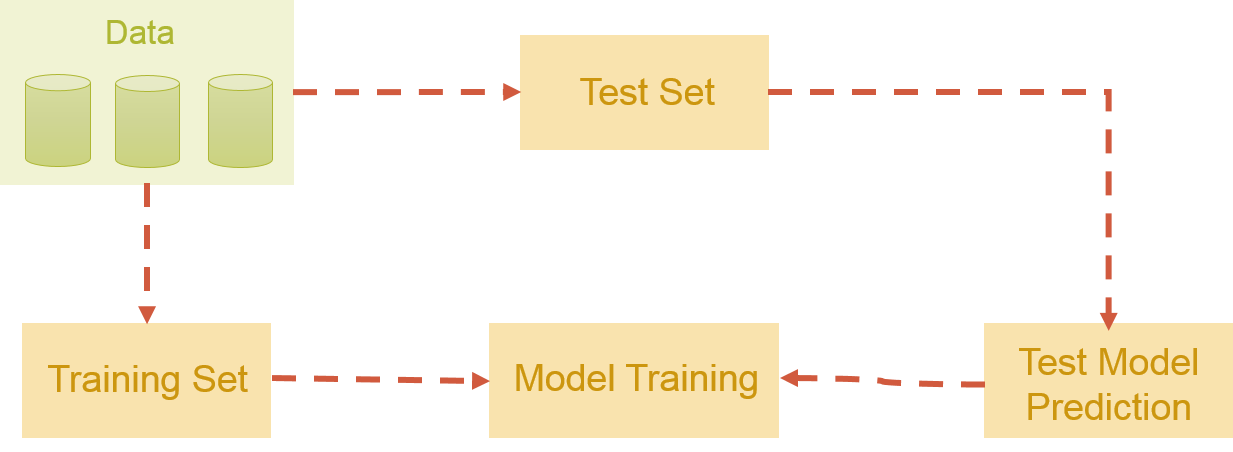
\includegraphics[width=12cm,height=10cm,keepaspectratio=true]{images/basic-ml-model.png}
	\caption{
		Basic supervised machine learning workflow.
	}
	\label{fig:basic-ml-model}
\end{figure}

\subsection{Unsupervised Learning}

In unsupervised learning, only the input variables are known and no corresponding output variables are known. Thus, no labels are given and the unsupervised machine learning algorithm is used to find the structure in the data i.e. finding hidden patterns to learn more about data. It is different from supervised learning in that, the correct output values are not known. Unsupervised learning is generally divided into clustering and association.

\begin{itemize}
	\item \textbf{Clustering}: Group objects in such a way that the similar objects placed in the same cluster.
	\item \textbf{Association}: Discover rules that define the large portions of the data such as people who buy product X may buy product Y as well.
\end{itemize}

The objective of machine learning is to analyze the past and present data and predict or make a decision for the future data. Machine learning is generally powered by a huge amount of data, which is generally referred as Big Data. It is generally defined as a too big or complex data, which cannot be processed on a single machine. As the data is growing day by day, the new tools are also required to process that big data on multiple machines and to extract the useful insights from the data.


One of the problems with the traditional machine learning model is the feature extraction challenge. The model designer or the programmer needs to specifically tell the model which features it should consider while making a decision. The model heavily relies on the programmer's understanding of data and this was a huge burden on the programmers. For problems like object recognition and language translation, it is considered as a huge and complicated problem.

Deep learning can be applied to extract features. They have the capability to focus only on the right features by themselves from big data while require very little input from the programmer. Deep learning models become a powerful tool in the current machine learning era.


\section{Artificial Neural Networks}
Artificial neural networks (ANNs) are generally inspired by the biological neural networks that mimic brain functionality \cite{wiki:ann}. These systems generally learnt by considering examples instead of specifically define rules for certain situations or cases. An ANN is a network of nodes, called artificial neurons, which are connected to other neurons using a link called \textit{synapse}. Each neuron gets the input, processes the input and passes the output to the next neuron.
In the most basic state, ANN consists of 3 layers: input layer, hidden layer, and output layer.


\begin{figure}[htpb]
	\centering
	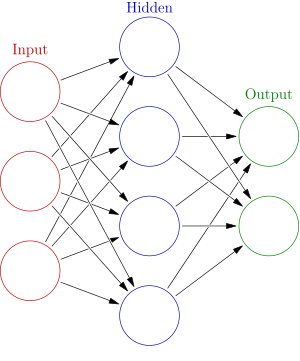
\includegraphics[width=6cm,height=10cm,keepaspectratio=true]{images/neural-net}
	\caption{
		An artificial neural network with three basic layers \cite{wiki:ann}.
	}
	\label{fig:wiki:ann}
\end{figure}


\subsection{Artificial Neuron}
An artificial neuron is the most basic unit of ANN. It takes inputs and produces an output. Generally, the inputs are multiplied by some weights in order to specify which inputs are more important. The higher the value of weight is, the more important it is. The inputs are shown as a, b, and c, and weights as $w_1$, $w_2$ and $w_3$ in Figure \ref{fig:single-neuron}. After then the products are summed together and passed to the activation function. So, if the summed value is greater than the threshold value of the activation function, the output is produced or in other terms, the neuron fired. In the other hand, no output is produced and neuron does not fire.

\begin{figure}[htpb]
	\centering
	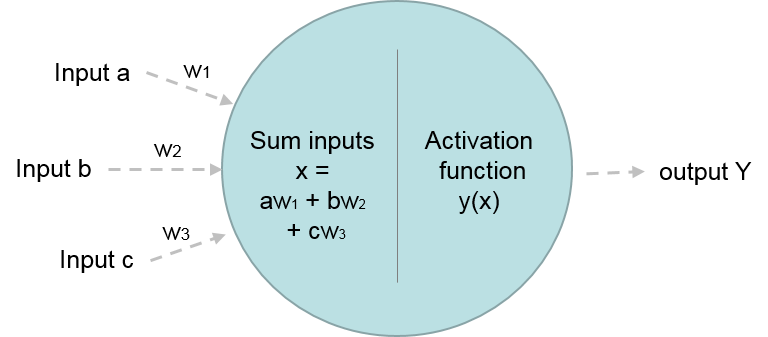
\includegraphics[width=10cm,height=10cm,keepaspectratio=true]{images/single-neuron}
	\caption{
		A single artificial neuron.
	}
	\label{fig:single-neuron}
\end{figure}

Artificial neurons adjust the weights as the learning proceeds and the process of finding weights is known as learning. ANN considers many different examples and finds the best possible combination of weights to provide the most accurate results. There are many other parameters involved to find a good combination of weights as well.

\subsection{Activation Function}

A function that takes an input and produces an output based on threshold value is known as activation function \cite{ujjwalkarn}. There are many activation functions available. Few of them are:

\subsubsection{Sigmoid}
It takes a real value input and scales it to the range of 0 to 1. It is also known as the logistic function. It is represented as:

\begin{equation} 
y = \frac{1}{1 + e^{-x}}
\end{equation}

Another variation of the sigmoid function is softmax function which is used for multiclass classification.

\subsubsection{Hyperbolic Tangent (Tanh)}
It takes a real value input and scales it to the range of -1 to 1. It is also a sigmoidal function as it also takes s-shaped.


\subsubsection{Rectified Linear Unit (ReLU)}
It stands for Rectified Linear Unit. It is the most used activation function with convolutional neural networks \cite{ujjwalkarn}. It takes the real value input and all negative values are mapped to zero. It is represented as:

\begin{center}
	$f(x) = max(0, x)$
\end{center}

\begin{figure}[htpb]
	\centering
	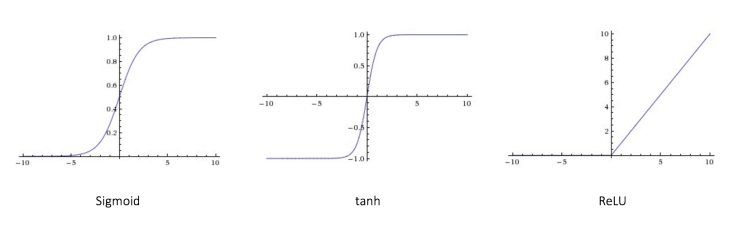
\includegraphics[width=15cm,height=10cm,keepaspectratio=true]{images/act-funcs}
	\caption{
		Activation functions \cite{ujjwalkarn}.
	}
	\label{fig:funcs}
\end{figure}

The graphs of all the activation functions are shown in Figure \ref{fig:funcs}.

\section{Convolutional Neural Network}
Convolutional neural network (CNN) is a class of deep neural network, which uses multilayer perceptrons. It consists of an input layer, an output layer, and multiple hidden layers. The hidden layers can be convolutional, pooling or fully connected layer. An example of CNN is shown in Figure \ref{fig:cnn_1d}. 

\begin{figure}[htpb]
	\centering
	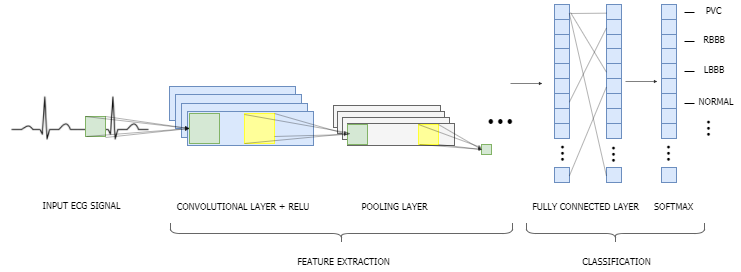
\includegraphics[width=15cm,height=15cm,keepaspectratio=true]{images/cnn_1d}
	\caption{
		Exacmpe of convolutional neural network.
	}
	\label{fig:cnn_1d}
\end{figure}

\subsection{Convolutional Layer}
In CNN, the first layer is always the convolutional layer. This layer applies a convolutional operation to the input and passes the output to the next layer. A filter (or sometimes referred as a kernel) is used which slides over all the areas of the input and extracts the features from it. The region where the filter is being applied at any instant of time is called as a receptive field. As the filter slides or convolves over the input signal, it multiples the filter with the original signal values (this can also be referred as element-wise multiplication) which results in a single value. The important point to note here is that this single result is just from a single receptive field. Therefore, the same operation will be carried out on other receptive fields by sliding the filter over different areas of the input signal. The filter can slide at any unit and this sliding unit is known as stride. Every unique area of the input signal will produce an output and the combined output together is called as feature map or an activation map.  If we assume that, the input size is 32x32, the filter size is 5x5 and the stride is 1 unit, then the size of the activation map will be 28x28. In a 2D array, the filter can be moved in both directions.

\subsection{Pooling Layer}
Pooling layer is used to downsample the convolutional layer output. There are several pooling options, for example, average pooling and $L_2$-norm pooling and max pooling, and the max pooling is the most popular. This layer basically takes a filter of size 2x2 with the same stride size. It then takes the largest of four numbers in the filter area. The same process is applied to the different subregions by sliding the filter all over the input. By convolving the filter around the input, it drastically reduces the spatial size of the input. The example of how pooling layer work is shown in Figure \ref{fig:maxpool}.

\begin{figure}[htpb]
	\centering
	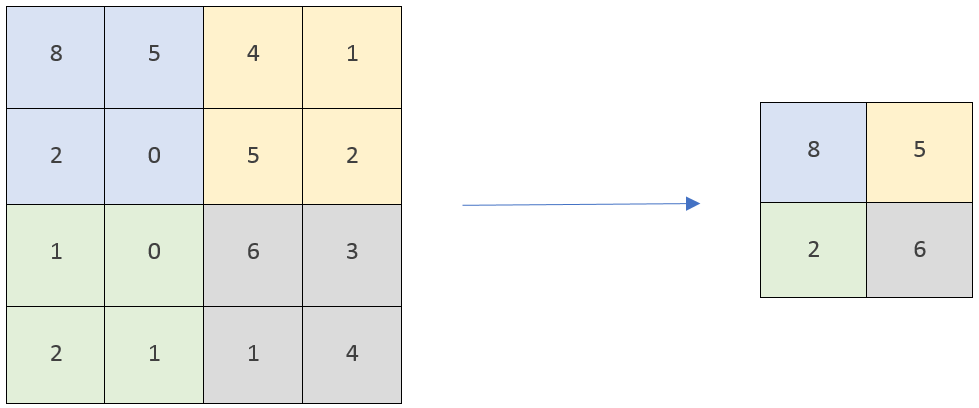
\includegraphics[width=12cm,height=10cm,keepaspectratio=true]{images/maxpool}
	\caption{
		Max pooling layer example.
	}
	\label{fig:maxpool}
\end{figure}

\subsection{Fully Connected Layer}
In a fully connected layer, the neurons of one layer are connected to all the neurons of the second layer, as shown in Figure \ref{fig:cnn_1d}. This layer can be seen in the regular neural network as well. The softmax function is applied to the output of the second layer. The output of the softmax function allows the probabilities for each label to be computed.

\section{Keras}

Keras is an open source artificial neural network library written in Python. It is very powerful and easy to use library for developing neural networks. It has a capability to run on top of TensorFlow, Microsoft Cognitive Toolkit (CNTK), or Theano, and can run on both CPU and GPU. Before the introduction of Keras, it was time-consuming to develop a network on TensorFlow or Theano. Keras supports both convolutional neural networks and recurrent neural network, as well as a combination of both.

The model starts by defining the model as sequential by calling a \textit{Sequential()} function of Keras, which is a linear stack of neural network layers. Then different types of layers are added into the model using \textit{add()} function. Keras supports almost all kinds of layers. The input dimensions are needed to specify when the layers are added to the model. Once the layers are added, the model is compiled by calling the \textit{compile()} function, which additionally needs 3 arguments.

\begin{itemize}
	\item Optimizer: It is used to optimize the neural network. Examples of optimizer are RSE, Adagrad and Adam.
	\item Loss Function: This is the value that model tries to minimize to calculate the error. For example, categorical cross-entropy and MSE.
	\item Metrics: It can be any existing metric or a custom defined metric function. But for classification problems metrics=['accuracy'] is recommended.
\end{itemize}

The model is trained by calling the \textit{fit()} method. This method lets the model iterate over the data and finds the most optimal neural network for the given data.

Keras has been used for training the CNN to identify cardiac arrhythmias.


\begin{figure}[htpb]
	\centering
	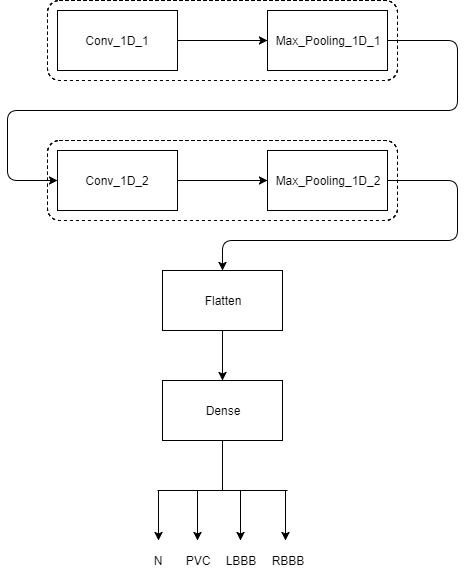
\includegraphics[width=20cm,height=15cm,keepaspectratio=true]{images/cnn_model}
	\caption{
		A 6-layer Convolutional Neural Network model for the identification of cardiac arrhythmia.
	}
	\label{fig:cnn_model}
\end{figure}


\section{Convolutional Neural Network for the Identification of Cardiac Arrhythmia}
A 6-layer Convolutional Neural Network (CNN) is used for the identification of arrhythmias from ECG signals. The trained model can detect 4 different kinds of ECG signals namely:

\begin{enumerate}
	\item Normal
	\item Left bundle branch block (LBBB)
	\item Right bundle branch block (RBBB)
	\item Premature ventricular contraction (PVC)
\end{enumerate}

The CNN layers are shown in Figure \ref{fig:cnn_model}.

\begin{figure}[htpb]
	\centering
	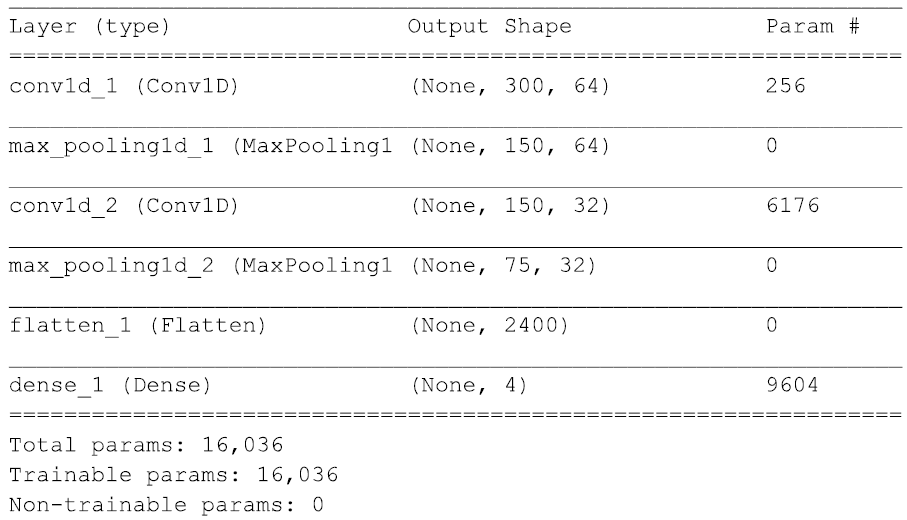
\includegraphics[width=12cm,height=10cm,keepaspectratio=true]{images/model_def_var}
	\caption{
		Layers used in the model and number of parameters to be optimized.
	}
	\label{fig:model_def_var_opt}
\end{figure}



\begin{figure}%
	\centering
	
	\subfigure[][]{%
		\label{fig:ex3-c}%
		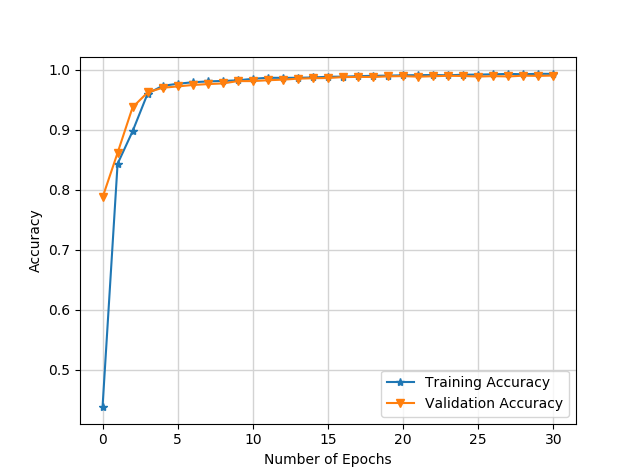
\includegraphics[height=4in]{images/acc}}%
	\hspace{8pt}%
	\subfigure[][]{%
		\label{fig:ex3-d}%
		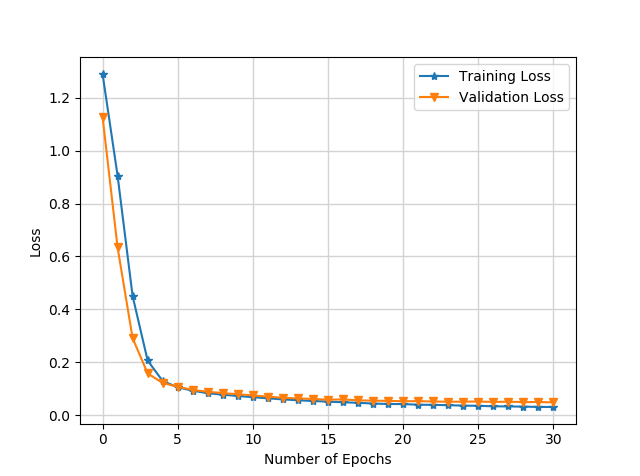
\includegraphics[height=4in]{images/val}}%
	\caption[A set of four subfigures.]{
		\subref{fig:ex3-c} Training and validation accuracy results
		\subref{fig:ex3-d} Training and validation loss function of CNN model for 30 iterations.}%
	\label{fig:acc_val}%
\end{figure}




\subsection{Layers Explanation}
The $1^{st}$ convolutional layer (Conv\_1D\_1) consists of 64 filters, whereas, the $2^{nd}$ convolutional layer (Conv\_1D\_2) consists of 32 filters with a kernel of size 3. The model needs to optimize total of 16,036 parameters in order to find an optimal CNN, as shown in Figure \ref{fig:model_def_var_opt}. For both convolutional layers, Rectified linear unit has been used as an activation function each followed by a max-pooling layer. The batch size of 1,000 was used for the training, along with the Adam algorithm to optimize the CNN. Since the model is trained for performing the classification of ECG signals, therefore, categorical cross-entropy loss function is used for calculating the loss of training and validation. After performing the convolutions, the flattening and dense layer has been used, followed by a softmax activation function to produce the final classification of 4 different classes.


The model is trained and tested for a number of iterations ranging from 10 to 100. The best model was found after 30 iterations. After that, the model remained stable with the slight improvement in the training as well as in the validation accuracy. The training and validation accuracy can be seen in Figure \ref{fig:acc_val}.



\subsection{Results}
The CNN model has achieved an accuracy of 99.2\% on MIT-BIH dataset. Total 16,415 ECG signals were extracted from the MIT-BIH dataset, out of which 10,998 (67\% of the total signals) were used for the training, and the remaining 5,417 (33\% of the total signals) were used for the validation of the model. The numbers for training and validation data can be seen in Table \ref{tab:train_count}. 

\renewcommand{\arraystretch}{2}
\begin{table}
	\caption{The numbers for training and validation data.} \label{tab:train_count}
	
	\begin{center}
		\begin{tabular}{ | l | r | r | }
			\hline
			\textbf{Type} & \textbf{Number of Training Data} & \textbf{Number of Validation Data}  \\ \hline
			Normal & 3,352 & 1,648\\ \hline
			LBBB  & 2,641 & 1,308  \\ \hline
			RBBB  & 2,498 & 1,285 \\ \hline
			PVC  & 2,507  & 1,176\\ \hline
			\textbf{Total}  & \textbf{10,998} &  \textbf{5,417} \\ \hline
		\end{tabular}
	\end{center}
	
\end{table}

During the validation of the model, 42 ECG signals were incorrectly classified from the overall 5,417 ECG signals. The result of false prediction is shown in Table \ref{tab:false_pred_count}. In the table, $a \rightarrow b$ represents that $a$ was classified as $b$.


\renewcommand{\arraystretch}{2}
\begin{table}
	\caption{The number of false prediction counts.} \label{tab:false_pred_count}
	
	\begin{center}
		\begin{tabular}{ | l | r | }
			\hline
			\textbf{False Prediction} & \textbf{Count} \\ \hline
			Normal $\rightarrow$ LBBB  & 1   \\ \hline
			Normal $\rightarrow$ RBBB  & 1  \\ \hline
			Normal $\rightarrow$ PVC  & 3  \\ \hline
			LBBB $\rightarrow$ PVC  & 6  \\ \hline
			RBBB $\rightarrow$ Normal  & 5  \\ \hline
			RBBB $\rightarrow$ PVC  & 3  \\ \hline
			PVC $\rightarrow$ Normal  & 9  \\ \hline
			PVC $\rightarrow$ LBBB  & 12 \\ \hline
			PVC $\rightarrow$ RBBB  & 2  \\ \hline
			\textbf{Total}   & \textbf{42}  \\ \hline
		\end{tabular}
	\end{center}
	
\end{table}